\documentclass[conference]{IEEEtran}
\IEEEoverridecommandlockouts
\usepackage{cite}
\usepackage{amsmath,amssymb,amsfonts}
\usepackage{algorithmic}
\usepackage{graphicx}
\usepackage{textcomp}
\usepackage{xcolor}
\usepackage{booktabs}
\usepackage{tikz}
\usetikzlibrary{shapes.geometric, arrows.meta, positioning, fit, backgrounds, calc, decorations.pathreplacing}
\def\BibTeX{{\rm B\kern-.05em{\sc i\kern-.025em b}\kern-.08em
    T\kern-.1667em\lower.7ex\hbox{E}\kern-.125emX}}

\begin{document}

\title{Multimodal Emotion Recognition via Causal-Diffusion Bridge (Affect-Diff)\\
{\footnotesize \textsuperscript{*}CISC 6080: Capstone Project in Data Science}}

\author{\IEEEauthorblockN{1\textsuperscript{st} [Ankit] [Sanjyal]}
\IEEEauthorblockA{\textit{Department of Computer Science - Data Science} \\
\textit{Fordham University}\\
New York, USA \\
email@fordham.edu}
}

\maketitle

\begin{abstract}
Emotion recognition plays a critical role in interpersonal social interactions, making it essential for robots and human-centered systems to correctly identify and respond to human emotions. While deep learning has significantly improved emotion classification from static images, multimodal emotion recognition (MER) in continuous video incorporating spatial, temporal, acoustic, and linguistic cues presents a more complex yet realistic challenge. Traditional fusion techniques often suffer from modality collapse, over-relying on dominant signals (such as text) and failing under real-world sensor noise or missing data. To address this, this project introduces Affect-Diff, a novel Causal-Diffusion Bridge architecture. We extract and fuse text, audio, and video modalities from the CMU-MOSEI dataset using a Causal Attention Graph and a Variational Autoencoder (VAE) bottleneck to form a robust joint latent space. By applying a 1D-UNet diffusion generative prior to this compressed space, the system acts as a powerful regularizer capable of mapping shared semantics and "healing" corrupted modalities, thereby enhancing the accuracy and resilience of emotion detection in multimodal environments.
\end{abstract}
\begin{IEEEkeywords}
Multimodal Emotion Recognition, Causal Inference, Diffusion Models, Variational Bottleneck, CMU-MOSEI, Robustness
\end{IEEEkeywords}

\section{Introduction}
Human communication is inherently complex and multimodal; we perceive and interpret emotion not only by listening to isolated words, but by also analyzing facial micro-expressions, body language, and vocal tone. In the rapidly expanding field of affective computing, utilizing machine learning with this human-like social intelligence is very essential. As artificial intelligence becomes increasingly integrated into human-centered systems such as healthcare monitoring, autonomous driving, and interactive robotics the ability to correctly identify and dynamically respond to human emotional states is now a necessity for safe and natural human-machine interaction.

While State-of-the-Art (SOTA) deep learning models achieve remarkable accuracy on clean, strictly controlled unimodal datasets, they are frequently inapplicable in real-world applications. A standard multimodal fusion model may crash, hallucinate predictions, or extremely degrade in performance if even a single sensory input is corrupted. We define this vulnerability as \textbf{Cascading Modality Failure}. In real-world environments, sensors are highly prone to degradation: a camera might fail in a dark room, a microphone could be overwhelmed by sudden wind noise, or a transcription algorithm might misinterpret heavily accented speech. Furthermore, standard multimodal architectures often suffer from \textit{modality collapse}, a phenomenon where the neural network lazily relies entirely on the statistically dominant modality (usually text) and ignores the acoustic and visual streams, rendering the multimodal design effectively useless when that primary stream fails.

This capstone project aims to address these critical vulnerabilities by building a multimodal emotion recognition (MER) system that mathematically mimics human intuition: specifically, the ability to dynamically assess uncertainty and trust one sense when another becomes unreliable. The goal of this project is to perform robust emotion classification by fusing linguistic, acoustic, and visual data streams using the CMU Multimodal Opinion Sentiment and Emotion Intensity (CMU-MOSEI) dataset. This dataset is the largest benchmark of its kind, containing 23,453 annotated video segments and providing rich, synchronized textual (GloVe), acoustic (COVAREP), and visual (FACET) features mapped to continuous sentiment scores and categorical Ekman emotion labels.

To overcome the limitations of standard late-fusion concatenation, this project proposes a novel architecture: \textbf{Affect-Diff}. Rather than passively combining features, our proposed analysis routes the extracted streams through a Causal Attention Graph and a Variational Autoencoder (VAE) bottleneck. This causal mechanism actively evaluates the directional influence and quality of each modality, down-weighting corrupted streams before they enter the joint latent space. Finally, we will implement a 1D-UNet diffusion generative prior to map this complex joint distribution. By analyzing the data through this generative lens, the diffusion model acts as a powerful regularizer that can "heal" or reconstruct missing modality data. The major sub-tasks of this project include writing custom data pre-processing scripts to bypass inherent dataset alignment bugs, coding the causal VAE bottleneck, and training the diffusion prior to achieve state-of-the-art robustness in multimodal emotion detection.

\section{Data Acquisition and Preprocessing}

\subsection{Data Source and Acquisition}
We utilize the \textbf{CMU-MOSEI} (CMU Multimodal Opinion Sentiment and Emotion Intensity) dataset \cite{zadeh2018mosei}, which remains the largest publicly available benchmark for multimodal sentiment analysis and emotion recognition. The corpus is collected ``in the wild'' from YouTube monologue videos and contains 23,453 annotated video segments (utterances) drawn from over 1,000 distinct speakers, ensuring substantial speaker and recording-condition diversity. The dataset is distributed under an academic research license via the CMU Multimodal Data SDK (\texttt{mmsdk}) Python package, which programmatically retrieves pre-extracted feature files from CMU servers as Computational Sequence Descriptors (\texttt{.csd}).

Three pre-extracted feature modalities are provided:
\begin{enumerate}
    \item \textbf{Text (Linguistic):} GloVe 6B 300-dimensional word embeddings \cite{zadeh2018mosei}, capturing distributional semantic relationships among transcribed words.
    \item \textbf{Audio (Acoustic):} COVAREP 74-dimensional feature vectors encoding fundamental frequency ($F_0$), voiced/unvoiced probability, spectral harmonics, glottal source parameters, and Mel-frequency cepstral coefficients (MFCCs), collectively capturing prosody, pitch contour, and vocal quality.
    \item \textbf{Video (Visual):} FACET 35-dimensional facial Action Unit (AU) intensity vectors derived from the VisualFacet42 toolkit, representing fine-grained facial micro-expressions (e.g., brow raise, lip corner pull).
\end{enumerate}

Each segment is densely annotated with a continuous sentiment score $s \in [-3, 3]$ (highly negative to highly positive) and intensity scores $e_k \in [0, 3]$ for the six Ekman basic emotions: \emph{Happy}, \emph{Sad}, \emph{Angry}, \emph{Fear}, \emph{Disgust}, and \emph{Surprise}. For categorical emotion recognition, we derive the discrete label as $y = \arg\max_k \, e_k$, converting the six-way intensity annotation into a single ground-truth class per segment.

\subsection{Dataset Statistics}
Table~\ref{tab:dataset_stats} summarizes the key statistics of the processed dataset. After our custom alignment and corrupted-entry pruning pipeline (described in Section~\ref{sec:preprocessing}), the usable corpus reduces from 23,453 raw segments to 3,292 aligned samples. We partition these into training, validation, and test splits at a 70/15/15 ratio using a fixed random permutation (seed = 42) to ensure reproducibility.

\begin{table}[htbp]
\caption{CMU-MOSEI Dataset Statistics After Alignment and Pruning}
\begin{center}
\begin{tabular}{@{}lr@{}}
\toprule
\textbf{Property} & \textbf{Value} \\
\midrule
Raw annotated segments & 23,453 \\
Distinct speakers & $>1{,}000$ \\
Aligned \& pruned samples & 3,292 \\
Training set & 2,304 (70\%) \\
Validation set & 494 (15\%) \\
Test set & 494 (15\%) \\
\midrule
Text feature dimension & 300 (GloVe) \\
Audio feature dimension & 74 (COVAREP) \\
Video feature dimension & 35 (VisualFacet42) \\
Sequence length (padded) & 50 time steps \\
\midrule
Number of emotion classes & 6 \\
Emotion taxonomy & Ekman basic emotions \\
\bottomrule
\end{tabular}
\label{tab:dataset_stats}
\end{center}
\end{table}

\subsection{Special Issues: Missing Values, Corruption, and Class Imbalance}
\label{sec:special_issues}
Working with in-the-wild multimodal data introduces several non-trivial quality issues that required engineering interventions beyond standard machine learning pipelines:

\textbf{(1) Corrupted and Misaligned Entries.}
The \texttt{mmsdk} feature files contain numerous video IDs where the temporal interval count does not match the feature matrix row count, causing dimension crashes during alignment. The default \texttt{mmsdk.mmdatasdk.computational\_sequence.alignment} routines frequently truncate or silently drop temporal frames, destroying resolution. We found that directly invoking the SDK's alignment function produced corrupted tensors for a substantial fraction of segments.

\textbf{(2) Missing Values (NaN Contamination).}
Several modality streams contain NaN entries arising from feature extraction failures (e.g., FACET produces NaN when no face is detected in a frame). If propagated into the network, these NaNs cascade through matrix multiplications and softmax operations, collapsing all gradient updates.

\textbf{(3) Variable Sequence Lengths.}
Utterances range from a single word to lengthy monologues, yielding highly variable temporal extents across the three modalities. Without uniform-length tensors, mini-batch collation for GPU training is impossible.

\textbf{(4) Feature Scale Disparity.}
The three modality streams occupy vastly different numerical ranges: GloVe vectors are pre-normalized to roughly unit scale, COVAREP features include raw $F_0$ values exceeding $300$\,Hz, and FACET AU intensities range from $0$ to $\sim$$5$. Without harmonization, the higher-energy modality dominates gradient flow during fusion, causing gradient vanishing for the remaining streams within the Variational Autoencoder bottleneck.

\textbf{(5) Class Imbalance.}
Because labels are derived via $\arg\max$ over six continuous intensity annotations, the resulting categorical distribution is skewed---\emph{Happy} and \emph{Sad} are over-represented relative to \emph{Fear} and \emph{Surprise}, which are inherently rarer in monologue-style YouTube content. Without mitigation, the classifier converges to a majority-class prior.

\subsection{Preprocessing Pipeline}
\label{sec:preprocessing}
We implement a multi-stage preprocessing pipeline that addresses each of the issues identified in Section~\ref{sec:special_issues}:

\textbf{Stage 1: Custom Index Unification and Corrupted Entry Pruning.}
Rather than relying on the default \texttt{mmsdk} alignment, we load each \texttt{.csd} file independently and compute the intersection of all video IDs that appear across the text, audio, video, and label modalities. For each candidate video ID, we verify that the temporal interval array length matches the feature matrix row count. Segments where this invariant is violated are pruned, preventing downstream dimension-mismatch errors.

\textbf{Stage 2: Manual Feature Extraction with Temporal Padding.}
For each valid video ID, we extract the feature matrices from all three modalities and the emotion intensity label vector. Sequences shorter than the target length $L = 50$ are zero-padded; sequences longer than $L$ are truncated to the first 50 time steps. This yields uniform tensors of shape $(L, D_m)$ for modality $m \in \{T, A, V\}$, enabling standard mini-batch collation.

\textbf{Stage 3: NaN Sanitization.}
All NaN and Inf values in the extracted feature tensors are replaced with zero via \texttt{torch.nan\_to\_num()} at the input boundary of the model's forward pass. This zero-imputation is a conservative choice that effectively treats missing frames as uninformative rather than introducing hallucinated feature values.

\textbf{Stage 4: Deterministic Train/Validation/Test Split.}
The 3,292 pruned samples are shuffled with a fixed random permutation (NumPy seed = 42) and partitioned into non-overlapping splits of 2,304 / 494 / 494 samples. Because the original CMU-MOSEI does not provide a standard speaker-disjoint split for the 6-way emotion task, we adopt this random partition and fix the seed for full reproducibility.

\subsection{Data Augmentation}
To combat overfitting on the relatively small training set (2,304 samples), we apply on-the-fly GPU-side augmentations during training only:

\textbf{(1) Temporal Frame Masking.}
Each temporal frame is independently zeroed out with probability $p_{\text{mask}} = 0.1$, simulating sporadic sensor dropout. This is applied to all three modalities.

\textbf{(2) Gaussian Noise Injection.}
Additive i.i.d.\ Gaussian noise $\mathcal{N}(0, \sigma^2 I)$ with $\sigma = 0.01$ is added to the audio and video feature streams, simulating sensor jitter. Text features are excluded from noise injection because adding continuous noise to discrete GloVe embeddings is semantically meaningless.

\textbf{(3) Stochastic Modality Dropout.}
During training, each modality is independently zeroed out with probability $p_{\text{drop}} = 0.1$, forcing the network to learn robust representations that do not catastrophically depend on any single input stream. This augmentation directly targets the modality collapse failure mode described in Section~\ref{sec:special_issues}.

\section{Related Work}
Multimodal Emotion Recognition (MER) has rapidly changed, moving from highly regulated, unimodal acoustic models to complex, real-world multimodal architectures. We review recent developments in three key areas generative diffusion models, causal inference for modality debiasing, and foundational MER methodologies in order to put the suggested Affect-Diff framework into context.

\subsection{Evolution of Multimodal Emotion Recognition}
Recent  studies emphasize a significant change in the manner in which MER systems handle physiological and audiovisual signals. Kumar et al. (2025) \cite{kumar2025survey} present a comprehensive taxonomy of MER development, examining benchmark datasets like RAVDESS, IEMOCAP, and DEAP. The authors detail the shift from traditional, manual feature extraction (such as HOG and LBP for video) and conventional Support Vector Machines to automated deep representation learning with 3D-CNNs and Vision Transformers predicting specific emotional outcomes. Importantly, they recognize the constraints of clean, lab-generated datasets when used in practical scenarios. In the same vein, Wu et al. (2024) \cite{wu2024survey} examine MER from a biomimetic perspective, analyzing datasets such as MOSEI and IEMOCAP. Their uniqueness is in framing MER as a bio-inspired sensing approach that replicates how humans effortlessly integrate multisensory signals (speech, visual, and text elements) to convey categorical emotions. This biologically-based viewpoint rationalizes our shift from basic late-fusion concatenation; rather, it supports our method of directing features into a unified, compressed latent space (the VAE bottleneck).

To evaluate our architecture, we rely on the foundational research by Zadeh et al. (2018) \cite{zadeh2018mosei}, who first presented the CMU-MOSEI dataset. Their approach used a Memory Fusion Network (an LSTM-based framework) to analyze GloVe word embeddings, COVAREP acoustic characteristics, and FACET visual features in order to forecast continuous sentiment and Ekman emotion classifications. Although we utilize their dataset, features, and targets, we acknowledge that their LSTM-driven temporal approach faces challenges with long-term misalignment and modality collapse. As a result, we substitute their architecture with our Causal-Diffusion bridge, employing tailored Z-normalization as a pre-processing step to harmonize the varying energy scales of the GloVe, COVAREP, and FACET features.

\subsection{Causal Inference and Modality Debiasing}
A constant issue in typical fusion networks is modality collapse, which occurs when the network heavily depends on a dominant signal (like text) and neglects the rest. Recent studies have applied causal inference to address this. A 2024 study on ``CausalMER'' \cite{causalmer2024} assesses this using the IEMOCAP and MSP-Podcast datasets. They derive particular acoustic features (eGeMAPS), visual characteristics (Action Units through OpenFace), and textual representations (RoBERTa embeddings) to forecast categorical emotion outcomes. Their pre-processing included rigorous temporal alignment and specific standardization by modality prior to using counterfactual reasoning and structural causal graphs. Their methodology's novel contribution lies in calculating and subtracting the “direct modality effect,” which prevents any one dominant modality from skewing the network. We directly incorporate this philosophy into our project. Incorporating a \texttt{CausalAttentionGraph} prior to our variational bottleneck allows us to dynamically calculate the directional impact of every input stream. If the visual or auditory stream is compromised, our graph automatically reduces its causal impact.

\subsection{Generative Diffusion for Missing Modalities}
Recently, diffusion models have been modified for sequential affective computing to address sensor noise and absent data. A key study from 2024 presented the Incomplete Multimodality-Diffused Emotion Recognition (IMDer) framework \cite{imder2024}, assessed using the IEMOCAP dataset. Employing Wav2Vec 2.0 (audio) and BERT (text) features aligned with specific emotion labels, their preprocessing included deliberately masking modalities to replicate missing data. They employed a score-driven diffusion model to translate Gaussian noise straight into the distribution space of the absent modalities. Expanding on this, the Multi-Condition Guided Diffusion Network (McDiff) \cite{mcdiff2025} was assessed using the IEMOCAP and MELD datasets, deriving utterance-level conversational embeddings (text, audio, video) to focus on utterance-level emotion categories, utilizing contextual Transformer pre-processing.

In the same vein, the Modality-Aware Diffusion Distillation Network (MDDN) \cite{mddn2025} employed the CMU-MOSI and CMU-MOSEI datasets, focusing on continuous sentiment ratings by leveraging GloVe, COVAREP, and FACET features, with temporal alignment and distillation mapping serving as crucial pre-processing stages. The 2025 ICCV paper on MD$^2$N \cite{md2n2025} primarily focuses on emotion classification for CMU-MOSEI and IEMOCAP utilizing ViT (visual) and wav2vec (acoustic) features. By utilizing pre-processing techniques such as duplex masking and cross-modal alignment, it emphasizes the crucial problem of "modality generation bias," demonstrating that diffusion priors can enhance stability in cross-modal reconstruction. These confirmed innovations provide the precise theoretical basis for the concluding phase of our Affect-Diff framework. Through the application of a 1D-UNet diffusion prior to our causal bottleneck space, we allow the model to mathematically recreate corrupted modality data during inference, guaranteeing reliable classification even during successive sensor failures

\section{Methods}
\label{sec:methods}
The Affect-Diff architecture introduces a \emph{Causal-Diffusion Bridge} that jointly trains five interacting subsystems under a single multi-task objective. This section describes each component in detail, followed by the composite loss function and the training procedure.

\subsection{Architectural Overview}
Given a temporally aligned triplet of feature sequences $(\mathbf{x}^T, \mathbf{x}^A, \mathbf{x}^V)$ with $\mathbf{x}^m \in \mathbb{R}^{L \times D_m}$, the end-to-end pipeline proceeds through five stages: (1)~modality-specific encoding, (2)~causal graph learning over unimodal representations, (3)~cross-modal fusion followed by variational compression into a joint latent space, (4)~a conditional denoising diffusion prior operating on the latent manifold, and (5)~task classification via attention pooling.  An auxiliary reconstruction decoder provides an additional gradient signal to prevent posterior collapse.  Every component beyond the encoder and classifier is togglable via configuration flags, enabling systematic ablation studies.  Fig.~\ref{fig:architecture} illustrates the complete end-to-end pipeline.

\begin{figure}[t]
\centering
\resizebox{\columnwidth}{!}{%
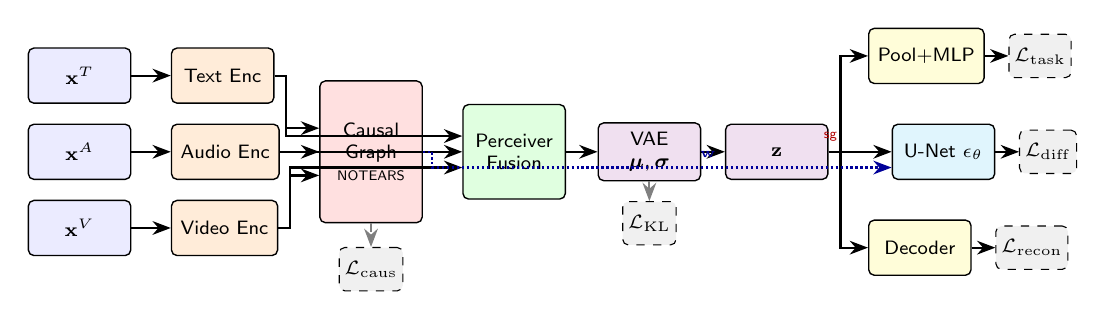
\begin{tikzpicture}[
    >=Stealth,
    node distance=0.35cm and 0.5cm,
    box/.style={draw, rounded corners=2pt, minimum height=0.7cm, minimum width=1.3cm,
                font=\scriptsize\sffamily, align=center, line width=0.5pt},
    inputbox/.style={box, fill=blue!8},
    encbox/.style={box, fill=orange!15},
    causalbox/.style={box, fill=red!12},
    fusionbox/.style={box, fill=green!12},
    vaebox/.style={box, fill=violet!12},
    diffbox/.style={box, fill=cyan!12},
    headbox/.style={box, fill=yellow!15},
    lossbox/.style={draw, rounded corners=2pt, fill=gray!12, dashed, font=\scriptsize\sffamily,
                    minimum height=0.55cm, align=center, inner sep=2pt},
    arr/.style={->, thick},
    darr/.style={->, thick, dashed, gray},
]

% === Column 1: Inputs ===
\node[inputbox] (xt) {$\mathbf{x}^T$};
\node[inputbox, below=0.25cm of xt] (xa) {$\mathbf{x}^A$};
\node[inputbox, below=0.25cm of xa] (xv) {$\mathbf{x}^V$};

% === Column 2: Encoders ===
\node[encbox, right=0.5cm of xt] (et) {Text Enc};
\node[encbox, right=0.5cm of xa] (ea) {Audio Enc};
\node[encbox, right=0.5cm of xv] (ev) {Video Enc};

\draw[arr] (xt) -- (et);
\draw[arr] (xa) -- (ea);
\draw[arr] (xv) -- (ev);

% === Column 3: Causal Graph ===
\node[causalbox, right=0.5cm of ea, minimum height=1.8cm] (cg) {Causal\\Graph\\{\tiny NOTEARS}};

\draw[arr] (et.east) -- ++(0.15,0) |- ([yshift=0.3cm]cg.west);
\draw[arr] (ea.east) -- (cg.west);
\draw[arr] (ev.east) -- ++(0.15,0) |- ([yshift=-0.3cm]cg.west);

% === Column 4: Fusion ===
\node[fusionbox, right=0.5cm of cg, minimum height=1.2cm] (fus) {Perceiver\\Fusion};

\draw[arr] (et.east) -- ++(0.15,0) |- ([yshift=0.2cm]fus.west);
\draw[arr] (ea.east) -- ++(0.25,0) |- (fus.west);
\draw[arr] (ev.east) -- ++(0.15,0) |- ([yshift=-0.2cm]fus.west);

% === Column 5: VAE ===
\node[vaebox, right=0.4cm of fus] (vae) {VAE\\$\boldsymbol{\mu}, \boldsymbol{\sigma}$};
\node[vaebox, right=0.3cm of vae] (znode) {$\mathbf{z}$};

\draw[arr] (fus) -- (vae);
\draw[arr] (vae) -- (znode);

% === Three output branches (stacked vertically to the right of z) ===
% Top: classifier
\node[headbox, above right=0.5cm and 0.5cm of znode] (cls) {Pool+MLP};
\node[lossbox, right=0.3cm of cls] (ltask) {$\mathcal{L}_{\mathrm{task}}$};

% Middle: diffusion
\node[diffbox, right=0.8cm of znode] (unet) {U-Net $\epsilon_\theta$};
\node[lossbox, right=0.3cm of unet] (ldiff) {$\mathcal{L}_{\mathrm{diff}}$};

% Bottom: reconstruction
\node[headbox, below right=0.5cm and 0.5cm of znode] (dec) {Decoder};
\node[lossbox, right=0.3cm of dec] (lrecon) {$\mathcal{L}_{\mathrm{recon}}$};

\draw[arr] (znode.east) -- ++(0.15,0) |- (cls.west);
\draw[arr] (znode.east) -- ++(0.15,0) coordinate (sg) -- (unet.west);
\draw[arr] (znode.east) -- ++(0.15,0) |- (dec.west);

% sg label
\node[font=\tiny\sffamily\color{red!70!black}, above left=0.01cm and -0.08cm of sg] {sg};

\draw[arr] (cls) -- (ltask);
\draw[arr] (unet) -- (ldiff);
\draw[arr] (dec) -- (lrecon);

% === Auxiliary losses ===
\node[lossbox, below=0.25cm of vae] (lkl) {$\mathcal{L}_{\mathrm{KL}}$};
\node[lossbox, below=0.3cm of cg] (lcaus) {$\mathcal{L}_{\mathrm{caus}}$};
\draw[darr] (vae.south) -- (lkl.north);
\draw[darr] (cg.south) -- (lcaus.north);

% === Causal weights to UNet ===
\draw[arr, densely dotted, blue!60!black] (cg.east) -- ++(0.12,0) |- ([yshift=-0.2cm]unet.west)
    node[pos=0.8, font=\tiny\sffamily, above, blue!60!black] {$\mathbf{w}$};

\end{tikzpicture}%
}
\caption{Affect-Diff architecture. Multimodal features are encoded, routed through a Causal Attention Graph (Stage~2) and Perceiver fusion into a VAE latent space (Stage~3). The latent $\mathbf{z}$ branches to: a classifier (Stage~5), a stop-gradiented U-Net diffusion prior conditioned on causal weights $\mathbf{w}$ (Stage~4), and a reconstruction decoder. Dashed arrows denote auxiliary losses.}
\label{fig:architecture}
\end{figure}

\subsection{Unimodal Encoders}
Each modality is processed by a dedicated encoder that maps raw pre-extracted features to a shared hidden dimension $H = 512$:

\textbf{Text Encoder.}
GloVe embeddings $\mathbf{x}^T \in \mathbb{R}^{L \times 300}$ are projected to $\mathbb{R}^{L \times H}$ via a linear layer, augmented with sinusoidal positional encodings, and processed through a 3-layer Transformer encoder with 8 attention heads, $4H$-wide feed-forward networks, pre-norm architecture, and GELU activations.

\textbf{Audio Encoder.}
COVAREP features $\mathbf{x}^A \in \mathbb{R}^{L \times 74}$ first pass through a 1-D convolutional front-end (kernel size 5, padding 2) with GroupNorm and GELU activation to capture local acoustic patterns, followed by the same 3-layer Transformer backbone. This ``Conformer-lite'' design captures both local spectral structure and global prosodic context.

\textbf{Video Encoder.}
VisualFacet42 features $\mathbf{x}^V \in \mathbb{R}^{L \times 35}$ are processed identically to audio, with a narrower 1-D convolutional kernel (size 3, padding 1) to reflect the higher spatial locality of facial action units.

All three encoders output temporally resolved hidden representations $\mathbf{h}^m \in \mathbb{R}^{L \times H}$.  The architecture additionally supports a \emph{foundation encoder} mode that substitutes the legacy encoders with frozen RoBERTa, HuBERT, and CLIP-ViT backbones, projecting their outputs to the same shared dimension via learned linear heads.

\subsection{Causal Attention Graph}
\label{sec:causal_graph}
Before the unimodal representations are fused, we learn a differentiable directed acyclic graph (DAG) over the three modality nodes $\{T, A, V\}$ to quantify their directional causal influence (Fig.~\ref{fig:causal_graph}).  Each unimodal hidden sequence is mean-pooled over the temporal axis to obtain node embeddings $\bar{\mathbf{h}}^m \in \mathbb{R}^H$, which are then stacked into a node matrix $\mathbf{N} \in \mathbb{R}^{3 \times H}$.  Directed edge scores are computed via scaled dot-product attention:

\begin{figure}[t]
\centering
\resizebox{\columnwidth}{!}{%
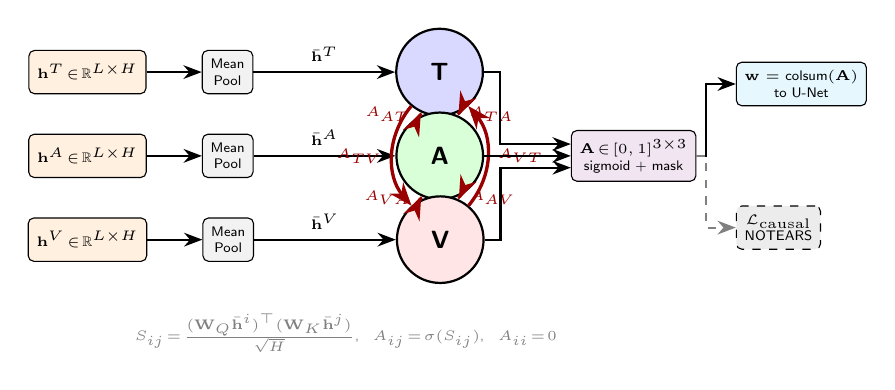
\begin{tikzpicture}[
    >=Stealth,
    node distance=1.8cm,
    modnode/.style={circle, draw, thick, minimum size=1.1cm, font=\small\sffamily\bfseries, inner sep=0pt},
    opbox/.style={draw, rounded corners=2pt, fill=gray!10, font=\tiny\sffamily, minimum height=0.55cm, align=center, inner sep=3pt},
    arr/.style={->, thick, >=Stealth},
    edgearr/.style={->, very thick, >=Stealth, red!60!black},
]

% === Unimodal inputs (left column) ===
\node[opbox, fill=orange!12] (ht) {$\mathbf{h}^T \!\in\! \mathbb{R}^{L \times H}$};
\node[opbox, fill=orange!12, below=0.5cm of ht] (ha) {$\mathbf{h}^A \!\in\! \mathbb{R}^{L \times H}$};
\node[opbox, fill=orange!12, below=0.5cm of ha] (hv) {$\mathbf{h}^V \!\in\! \mathbb{R}^{L \times H}$};

% === Mean pool ===
\node[opbox, right=0.7cm of ht] (pt) {Mean\\Pool};
\node[opbox, right=0.7cm of ha] (pa) {Mean\\Pool};
\node[opbox, right=0.7cm of hv] (pv) {Mean\\Pool};

\draw[arr] (ht) -- (pt);
\draw[arr] (ha) -- (pa);
\draw[arr] (hv) -- (pv);

% === Graph nodes ===
\node[modnode, fill=blue!15, right=1.8cm of pt] (T) {T};
\node[modnode, fill=green!15, right=1.8cm of pa] (A) {A};
\node[modnode, fill=red!10, right=1.8cm of pv] (V) {V};

\draw[arr] (pt) -- (T) node[midway, above, font=\tiny\sffamily] {$\bar{\mathbf{h}}^T$};
\draw[arr] (pa) -- (A) node[midway, above, font=\tiny\sffamily] {$\bar{\mathbf{h}}^A$};
\draw[arr] (pv) -- (V) node[midway, above, font=\tiny\sffamily] {$\bar{\mathbf{h}}^V$};

% === Directed edges (learned) with weight labels ===
\draw[edgearr, bend left=25] (T) to node[font=\tiny\sffamily, right, pos=0.5] {$A_{TA}$} (A);
\draw[edgearr, bend left=25] (A) to node[font=\tiny\sffamily, left, pos=0.5] {$A_{AT}$} (T);
\draw[edgearr, bend left=25] (A) to node[font=\tiny\sffamily, right, pos=0.5] {$A_{AV}$} (V);
\draw[edgearr, bend left=25] (V) to node[font=\tiny\sffamily, left, pos=0.5] {$A_{VA}$} (A);
\draw[edgearr, bend right=40] (T) to node[font=\tiny\sffamily, left, pos=0.5] {$A_{TV}$} (V);
\draw[edgearr, bend right=40] (V) to node[font=\tiny\sffamily, right, pos=0.5] {$A_{VT}$} (T);

% === Output: adjacency matrix ===
\node[opbox, fill=violet!10, right=1.1cm of A, minimum width=1.3cm] (adj) {$\mathbf{A} \!\in\! [0,1]^{3\times 3}$\\{\tiny sigmoid + mask}};
\draw[arr] (T.east) -- ++(0.2,0) |- ([yshift=0.15cm]adj.west);
\draw[arr] (A.east) -- (adj.west);
\draw[arr] (V.east) -- ++(0.2,0) |- ([yshift=-0.15cm]adj.west);

% === Outputs ===
\node[opbox, fill=cyan!10, above right=0.3cm and 0.5cm of adj] (wout) {$\mathbf{w} = \text{colsum}(\mathbf{A})$\\{\tiny to U-Net}};
\node[opbox, fill=gray!15, dashed, below right=0.3cm and 0.5cm of adj] (ldag) {$\mathcal{L}_{\mathrm{causal}}$\\{\tiny NOTEARS}};

\draw[arr] (adj.east) -- ++(0.12,0) |- (wout.west);
\draw[arr, dashed, gray] (adj.east) -- ++(0.12,0) |- (ldag.west);

% === Equation annotation ===
\node[font=\tiny\sffamily, text=gray, below=1.6cm of pa, xshift=1.5cm, align=center]
    {$S_{ij} \!=\! \frac{(\mathbf{W}_Q \bar{\mathbf{h}}^i)^\top (\mathbf{W}_K \bar{\mathbf{h}}^j)}{\sqrt{H}}$, \; $A_{ij} \!=\! \sigma(S_{ij})$, \; $A_{ii} \!=\! 0$};

\end{tikzpicture}%
}
\caption{Causal Attention Graph detail.  Unimodal encoder outputs are mean-pooled to node embeddings, then directed edge weights are computed via scaled dot-product attention with sigmoid activation.  Self-loops are masked to zero.  The soft adjacency matrix $\mathbf{A}$ yields modality importance weights $\mathbf{w}$ (fed to the U-Net) and a NOTEARS acyclicity penalty $\mathcal{L}_{\mathrm{causal}}$.}
\label{fig:causal_graph}
\end{figure}
\begin{equation}
    S_{ij} = \frac{(\mathbf{W}_Q \bar{\mathbf{h}}^i)^\top (\mathbf{W}_K \bar{\mathbf{h}}^j)}{\sqrt{H}}, \quad i \neq j
\end{equation}
where $\mathbf{W}_Q, \mathbf{W}_K \in \mathbb{R}^{H \times H}$ are learned projections and self-loops are masked to zero.  Edge probabilities are obtained via element-wise sigmoid, yielding a soft adjacency matrix $\mathbf{A} \in [0,1]^{3 \times 3}$.

To enforce acyclicity, we adopt the NOTEARS constraint \cite{zheng2018notears}:
\begin{equation}
    h(\mathbf{A}) = \mathrm{tr}\!\left(e^{\mathbf{A} \circ \mathbf{A}}\right) - d = 0
\end{equation}
where $d = 3$ is the number of nodes and $\circ$ denotes the Hadamard product.  This constraint is added to the training loss as a differentiable penalty.  Normalized column sums of $\mathbf{A}$ provide per-modality importance weights that are logged for interpretability and fed as conditioning signals to the diffusion model.

\subsection{Cross-Modal Fusion and Variational Bottleneck}
\label{sec:fusion_vae}
The three encoded sequences are fused into a single multimodal representation using a \textbf{Perceiver-style cross-modal attention} mechanism \cite{jaegle2021perceiver}.  A set of $L_b = 50$ learnable bottleneck tokens $\mathbf{B} \in \mathbb{R}^{L_b \times H}$ queries into the concatenated key-value sequence $[\mathbf{h}^T; \mathbf{h}^A; \mathbf{h}^V] \in \mathbb{R}^{3L \times H}$ through two alternating rounds of multi-head cross-attention and self-attention, each with pre-norm residual connections and $4H$-wide GELU feed-forward sub-layers.  Learnable modality-type embeddings are added to the key-value tokens so the attention mechanism can distinguish their origin.

The fused representation $\mathbf{F} \in \mathbb{R}^{L_b \times H}$ is projected to posterior parameters through linear heads:
\begin{equation}
    \boldsymbol{\mu} = \mathbf{W}_\mu \mathbf{F}, \quad \log \boldsymbol{\sigma}^2 = \mathrm{clamp}(\mathbf{W}_\sigma \mathbf{F},\, -10,\, 5)
\end{equation}
with $\boldsymbol{\mu}, \log \boldsymbol{\sigma}^2 \in \mathbb{R}^{L_b \times d_z}$ and latent dimension $d_z = 256$.  The clamping prevents numerical overflow under mixed-precision (fp16) training.  The latent code is sampled via the reparameterization trick:
\begin{equation}
    \mathbf{z} = \boldsymbol{\mu} + \boldsymbol{\epsilon} \odot \boldsymbol{\sigma}, \quad \boldsymbol{\epsilon} \sim \mathcal{N}(\mathbf{0}, \mathbf{I})
\end{equation}
At inference time, the deterministic mean $\boldsymbol{\mu}$ is used directly.  The KL divergence between the approximate posterior $q_\phi(\mathbf{z} \mid \mathbf{x})$ and the unit Gaussian prior $p(\mathbf{z}) = \mathcal{N}(\mathbf{0}, \mathbf{I})$ is regularized with a $\beta$-weighted free-bits objective \cite{kingma2016freebits}:
\begin{equation}
    \mathcal{L}_{\mathrm{KL}} = \beta \cdot \frac{1}{BL_b} \sum_{b,l} \sum_{d=1}^{d_z} \max\!\left(0,\; \mathrm{KL}_d^{(b,l)} - \lambda\right)
\end{equation}
where $\mathrm{KL}_d = -\frac{1}{2}(1 + \log\sigma_d^2 - \mu_d^2 - \sigma_d^2)$ is the per-dimension KL and $\lambda = 0.25$ nats is the free-bits threshold.  This formulation permits each latent dimension to encode up to $\lambda$ nats of information without penalty, preventing posterior collapse while ensuring zero loss when the posterior matches the prior.

\subsection{Conditional Denoising Diffusion Prior}
\label{sec:diffusion}
To learn the complex manifold of the aggregate posterior $q(\mathbf{z})$, we train a denoising diffusion probabilistic model (DDPM) \cite{ho2020ddpm} directly on the VAE latent space.  Critically, following Latent Diffusion Models \cite{rombach2022ldm}, the latent input to the diffusion model is \textbf{stop-gradiented}: $\mathbf{z}_{\text{diff}} = \mathrm{sg}(\mathbf{z})$.  This architectural choice prevents the diffusion loss from flowing back through the encoder, which we found empirically to create a conflicting gradient that degrades classification accuracy.

\textbf{Forward Process.}
Given a cosine noise schedule $\{\beta_t\}_{t=1}^{T}$ with $T = 1{,}000$ steps \cite{ho2020ddpm}, the forward process adds Gaussian noise:
\begin{equation}
    q(\mathbf{z}_t \mid \mathbf{z}_0) = \mathcal{N}\!\left(\mathbf{z}_t;\; \sqrt{\bar{\alpha}_t}\,\mathbf{z}_0,\; (1 - \bar{\alpha}_t)\mathbf{I}\right)
\end{equation}
where $\bar{\alpha}_t = \prod_{s=1}^{t}(1 - \beta_s)$.

\textbf{Noise Prediction Network.}
The reverse process is parameterized by a 1-D U-Net $\epsilon_\theta$ that predicts the noise added at each timestep.  The network follows a standard encoder-bottleneck-decoder topology with skip connections:
\begin{itemize}
    \item \emph{Input:} $\mathbf{z}_t \in \mathbb{R}^{d_z \times L_b}$ (channel-first format).
    \item \emph{Encoder:} Three resolution stages with channel multipliers $(1\times, 2\times, 4\times)$ relative to a base dimension of 128.  Each stage contains two residual blocks (Conv1d $\to$ GroupNorm $\to$ SiLU) followed by stride-2 downsampling.
    \item \emph{Bottleneck:} Two residual blocks at the coarsest resolution (512 channels).
    \item \emph{Decoder:} Symmetric upsampling stages with transposed convolutions and skip connections from the encoder.
\end{itemize}

The U-Net is \textbf{triply conditioned} via additive injection into every residual block:
\begin{equation}
    \mathbf{c} = \mathrm{MLP}_t(t) + \mathrm{Emb}_y(y) + \mathrm{MLP}_w(\mathbf{w})
\end{equation}
where $\mathrm{MLP}_t$ maps the sinusoidal timestep embedding to $\mathbb{R}^{512}$, $\mathrm{Emb}_y$ is a learned class embedding for the emotion label $y \in \{0, \ldots, 5\}$ (with an additional null token for classifier-free guidance), and $\mathrm{MLP}_w$ projects the 3-dimensional causal influence vector $\mathbf{w}$ (column sums of $\mathbf{A}$, detached from the graph) to the same conditioning dimension.

\textbf{Training Objective.}
The simplified DDPM loss is:
\begin{equation}
    \mathcal{L}_{\mathrm{diff}} = \mathbb{E}_{t, \boldsymbol{\epsilon}}\!\left[\left\| \boldsymbol{\epsilon} - \epsilon_\theta(\mathbf{z}_t, t, y, \mathbf{w}) \right\|^2\right]
\end{equation}
During training, classifier-free guidance (CFG) is implemented by randomly replacing the class label with the null token with probability 0.2.

\textbf{Inference Sampling.}
At test time, we use DDIM sampling \cite{song2021ddim} with 50 deterministic steps ($\eta = 0$) and a CFG scale of $s = 4.0$ for accelerated, high-fidelity generation.  An exponential moving average (EMA) copy of the U-Net weights ($\gamma_{\mathrm{EMA}} = 0.999$) is maintained and used during inference for improved sample quality.

\subsection{Reconstruction Decoder}
To ensure that the VAE latent space retains sufficient information about the original input features---rather than collapsing to a trivial posterior---we include a lightweight per-modality reconstruction decoder.  Three independent 2-layer MLPs (Linear $\to$ LayerNorm $\to$ GELU $\to$ Dropout $\to$ Linear) project the latent code $\mathbf{z} \in \mathbb{R}^{L_b \times d_z}$ back to the original feature dimensions:
\begin{equation}
    \hat{\mathbf{x}}^m = \mathrm{Dec}_m(\mathbf{z}), \quad m \in \{T, A, V\}
\end{equation}
The reconstruction loss is the average mean-squared error across modalities:
\begin{equation}
    \mathcal{L}_{\mathrm{recon}} = \frac{1}{3}\sum_{m \in \{T,A,V\}} \left\| \hat{\mathbf{x}}^m - \mathbf{x}^m \right\|_2^2
\end{equation}

\subsection{Task Classifier}
The latent sequence $\mathbf{z} \in \mathbb{R}^{L_b \times d_z}$ is compressed to a single vector via \textbf{learnable attention pooling}: a learned query token $\mathbf{q} \in \mathbb{R}^{d_z}$ attends to all $L_b$ positions through scaled dot-product attention:
\begin{equation}
    \bar{\mathbf{z}} = \mathrm{softmax}\!\left(\frac{\mathbf{q}\, \mathbf{z}^\top}{\sqrt{d_z}}\right) \mathbf{z} \;\in\; \mathbb{R}^{d_z}
\end{equation}
The pooled representation is fed to a two-layer MLP classifier (Linear(256,\,128) $\to$ LayerNorm $\to$ GELU $\to$ Dropout(0.3) $\to$ Linear(128,\,6)) producing logits over the six Ekman emotion classes.  The classification loss uses label-smoothed cross-entropy with smoothing parameter $\alpha = 0.1$ to mitigate overconfident predictions on the imbalanced label distribution.

\subsection{Joint Training Objective}
\label{sec:joint_loss}
The five loss components are combined with coefficient weighting and \textbf{curriculum warmup schedules} to stabilize early training:
\begin{equation}
    \mathcal{L} = \mathcal{L}_{\mathrm{task}} + \gamma_{\mathrm{kl}}\,\mathcal{L}_{\mathrm{KL}} + \gamma\,\lambda_d\,\mathcal{L}_{\mathrm{diff}} + \gamma\,\lambda_r\,\mathcal{L}_{\mathrm{recon}} + \lambda_c\,\mathcal{L}_{\mathrm{causal}}
\end{equation}
where $\lambda_d = 0.5$, $\lambda_r = 0.5$, $\lambda_c = 0.05$ are fixed coefficients and $\gamma$, $\gamma_{\mathrm{kl}}$ are epoch-dependent warmup ramps:
\begin{equation}
    \gamma = \min\!\left(1,\; \frac{\mathrm{epoch}}{20}\right), \quad \gamma_{\mathrm{kl}} = \min\!\left(1,\; \frac{\mathrm{epoch}}{30}\right)
\end{equation}
The classification loss receives no warmup and dominates early training, allowing the encoder to learn discriminative features before the auxiliary regularizers engage.  The KL warmup is deliberately slower (30 epochs vs.\ 20) to prevent early posterior collapse.

\subsection{Training Details}
\label{sec:training_details}
The entire model (72.8M parameters, 57.9M trainable) is trained end-to-end using PyTorch Lightning with the following configuration:

\begin{itemize}
    \item \textbf{Optimizer:} AdamW with learning rate $3 \times 10^{-4}$ and weight decay $10^{-5}$.
    \item \textbf{Scheduler:} Cosine annealing over 150 epochs with no warm restarts.
    \item \textbf{Precision:} Mixed fp16/fp32 (AMP) with dynamic loss scaling.  All loss summations and the KL computation are cast to fp32 to prevent overflow.
    \item \textbf{Hardware:} 2$\times$ NVIDIA V100 GPUs via PyTorch DDP with batch size 64 (32 per device).
    \item \textbf{Gradient Clipping:} Global $\ell_2$-norm clipping at 1.0 to prevent gradient explosions from the diffusion or causal penalty terms.
    \item \textbf{Early Stopping:} Patience of 30 epochs on validation loss.
    \item \textbf{Reproducibility:} All random seeds (PyTorch, NumPy, Python) fixed at 42.
\end{itemize}

\subsection{Customizations from Existing Models}
While Affect-Diff draws inspiration from several existing frameworks, the following architectural decisions represent novel customizations that distinguish our approach:

\begin{enumerate}
    \item \textbf{Stop-Gradient Diffusion (from Latent Diffusion Models):} Rombach et al.\ \cite{rombach2022ldm} train diffusion on a \emph{frozen} autoencoder.  We adapt this to a \emph{jointly trained} setting by applying $\mathrm{sg}(\cdot)$ to the latent input of the diffusion model, preserving end-to-end training of the encoder via the task and reconstruction losses while isolating it from conflicting diffusion gradients.

    \item \textbf{Triple Conditioning of the U-Net (from IMDer and McDiff):} Prior latent diffusion works \cite{imder2024, mcdiff2025} condition on timestep and class label only.  We additionally inject the learned causal influence vector $\mathbf{w}$ from the DAG, enabling the denoiser to be \emph{modality-aware}---producing higher-fidelity reconstructions for modalities that the causal graph identifies as reliable.

    \item \textbf{NOTEARS DAG Learning as a Fusion Pre-Filter (from CausalMER):} CausalMER \cite{causalmer2024} applies causal reasoning \emph{post hoc} via counterfactual subtraction.  We instead embed a differentiable NOTEARS \cite{zheng2018notears} graph directly into the forward pass \emph{before} fusion, allowing the learned edge weights to dynamically re-weight modality contributions on a per-sample basis during training.

    \item \textbf{Free-Bits KL with Separate Warmup:} Standard $\beta$-VAE \cite{higgins2017betavae} uses a single KL weight.  We combine threshold-based free bits \cite{kingma2016freebits} ($\lambda = 0.25$ nats per dimension) with a dedicated 30-epoch linear warmup that is decoupled from the auxiliary loss warmup, preventing both posterior collapse and early KL domination simultaneously.
\end{enumerate}
\begin{thebibliography}{00}

% --- Foundational & Survey Papers ---
\bibitem{wu2024survey} Y. Wu, Q. Mi, and T. Gao, ``A Comprehensive Review of Multimodal Emotion Recognition: Techniques, Challenges, and Future Directions,'' \textit{Biomimetics}, vol. 9, 2024.
\bibitem{kumar2025survey} M. J. D. Kumar, M. S. Rao, and K. C. Narendra, ``Multimodal Emotion Recognition: A Comprehensive Survey of Datasets, Methods, and Applications,'' \textit{IEEE Access}, vol. 13, 2025.
\bibitem{zadeh2018mosei} A. Zadeh et al., ``Multimodal Language Analysis in the Wild: CMU-MOSEI Dataset and Interpretable Dynamic Fusion Graph,'' in \textit{Proc. 56th Annual Meeting of the Association for Computational Linguistics}, 2018, pp. 2236--2246.

% --- Causal Inference & Debiasing ---
\bibitem{causalmer2024} ``Causal Inference for Modality Debiasing in Multimodal Emotion Recognition,'' \textit{Applied Sciences}, MDPI, vol. 14, no. 23, 2024.
\bibitem{zheng2018notears} X. Zheng, B. Aragam, P. K. Ravikumar, and E. P. Xing, ``DAGs with NO TEARS: Continuous Optimization for Structure Learning,'' in \textit{Advances in Neural Information Processing Systems (NeurIPS)}, 2018, pp. 9472--9483.

% --- Diffusion Models for Missing Modalities ---
\bibitem{imder2024} ``Incomplete Multimodality-Diffused Emotion Recognition,'' \textit{OpenReview}, 2024.
\bibitem{mcdiff2025} ``Multi-Condition Guided Diffusion Network for Multimodal Emotion Recognition in Conversation,'' \textit{Findings of the Association for Computational Linguistics (NAACL)}, 2025.
\bibitem{mddn2025} ``Modality-Aware Diffusion Distillation Network for Sentiment Analysis,'' \textit{IEEE Transactions}, 2025.
\bibitem{md2n2025} ``Unbiased Missing-Modality Multimodal Learning,'' in \textit{Proc. IEEE/CVF International Conference on Computer Vision (ICCV)}, 2025.

% --- Core Deep Learning Methods ---
\bibitem{ho2020ddpm} J. Ho, A. Jain, and P. Abbeel, ``Denoising Diffusion Probabilistic Models,'' in \textit{Advances in Neural Information Processing Systems (NeurIPS)}, 2020, pp. 6840--6851.
\bibitem{song2021ddim} J. Song, C. Meng, and S. Ermon, ``Denoising Diffusion Implicit Models,'' in \textit{Proc. International Conference on Learning Representations (ICLR)}, 2021.
\bibitem{rombach2022ldm} R. Rombach, A. Blattmann, D. Lorenz, P. Esser, and B. Ommer, ``High-Resolution Image Synthesis with Latent Diffusion Models,'' in \textit{Proc. IEEE/CVF Conference on Computer Vision and Pattern Recognition (CVPR)}, 2022, pp. 10684--10695.
\bibitem{jaegle2021perceiver} A. Jaegle et al., ``Perceiver: General Perception with Iterative Attention,'' in \textit{Proc. International Conference on Machine Learning (ICML)}, 2021, pp. 4651--4664.
\bibitem{higgins2017betavae} I. Higgins et al., ``$\beta$-VAE: Learning Basic Visual Concepts with a Constrained Variational Framework,'' in \textit{Proc. International Conference on Learning Representations (ICLR)}, 2017.
\bibitem{kingma2016freebits} D. P. Kingma, T. Salimans, R. Jozefowicz, X. Chen, I. Sutskever, and M. Welling, ``Improved Variational Inference with Inverse Autoregressive Flow,'' in \textit{Advances in Neural Information Processing Systems (NeurIPS)}, 2016, pp. 4743--4751.

\end{thebibliography}

\end{document}
